% Source page: Deepfield.md Page 7; exactly one frame.
\setsource{\href{https://doi.org/10.1038/s41586-026-10644-y}{Co-Scientist, Nature (2026)}}
\begin{frame}[c,label=md-7]{Co-Scientist: focus on generating hypotheses}
\small
\textbf{Core reasoning steps}
\begin{enumerate}
    \setlength{\itemsep}{0.2em}
    \item Multi-agent self-play scientific debate
    \item Tournament-based hypothesis comparison and ranking
    \item Evolution with meta-review and refinement
\end{enumerate}
\smallskip
\begin{figure}
\centering
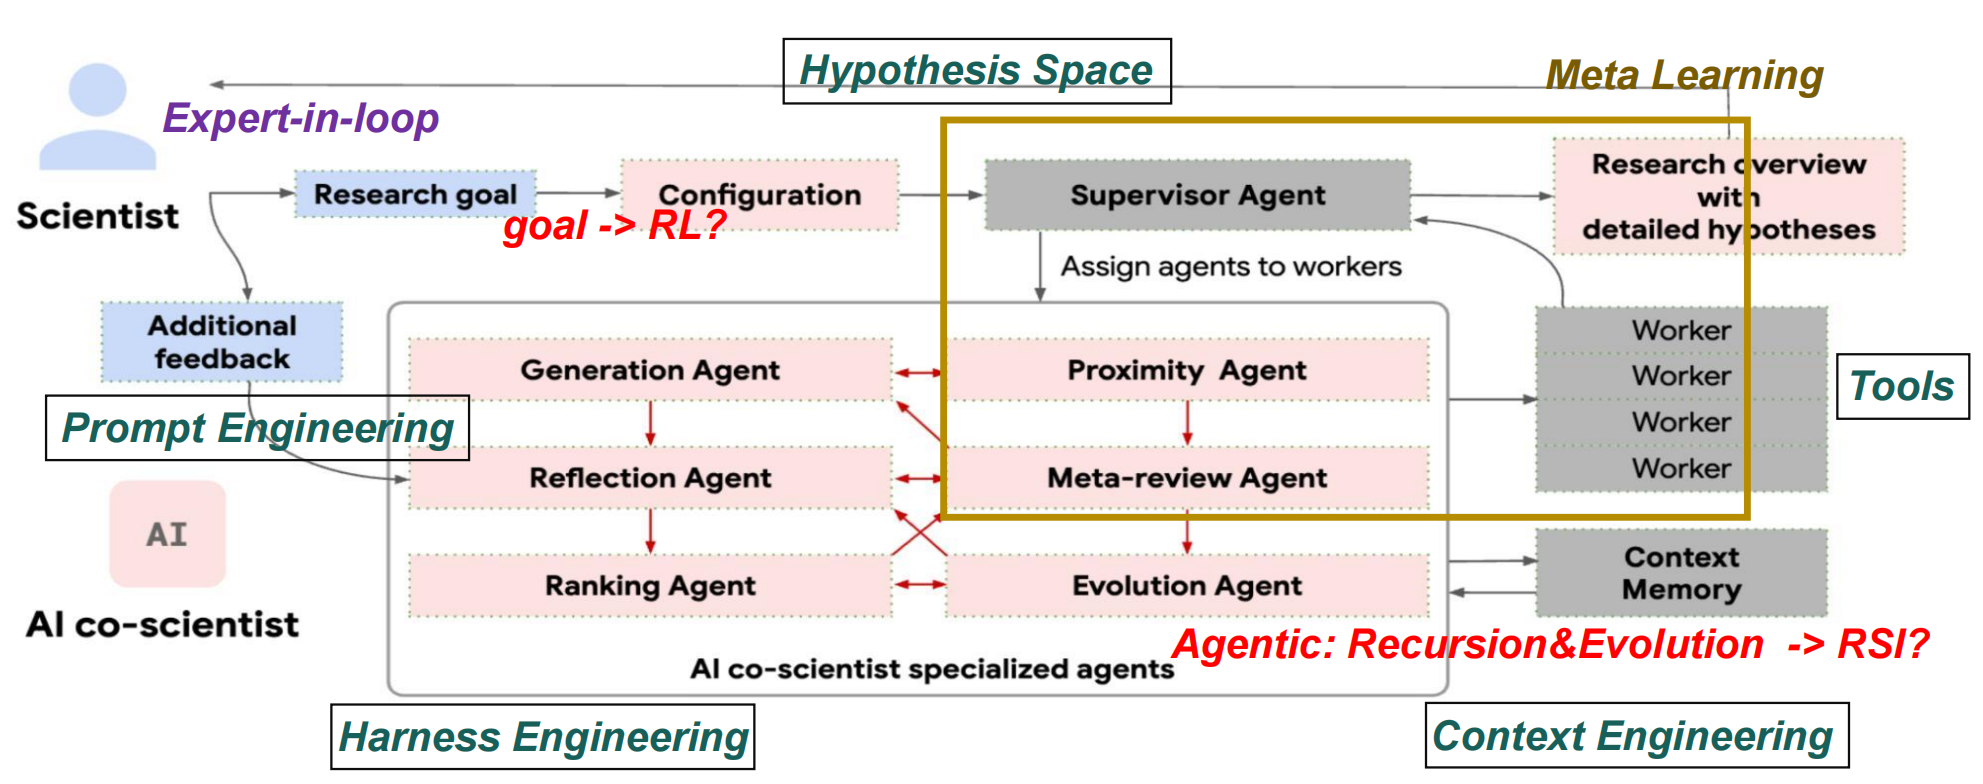
\includegraphics[width=0.86\textwidth]{architecture_co_scientist_with notes.png}
\caption{Co-Scientist architecture with annotated research concepts.}
\end{figure}
\note{The Introduction describes three thinking and reasoning steps:
scientific debate generates hypotheses; tournament comparisons rank them;
hypothesis evolution generates improved candidates. These are mechanisms
within the broader test-time compute scaling paradigm. The paper separately
describes agentic self-critique and tool use as supporting capabilities.
The abstract groups the technical contributions into an asynchronous
multi-agent architecture and a tournament evolution process.}
\end{frame}

% Source page: Deepfield.md Page 8; scaling and open question on separate frames.
\setsource{\href{https://www.nature.com/articles/s41586-026-10644-y}{Co-Scientist, Nature (2026)}}
\begin{frame}[c,label=md-8]{Co-Scientist: test-time compute scaling}
\footnotesize
\begin{figure}
\centering
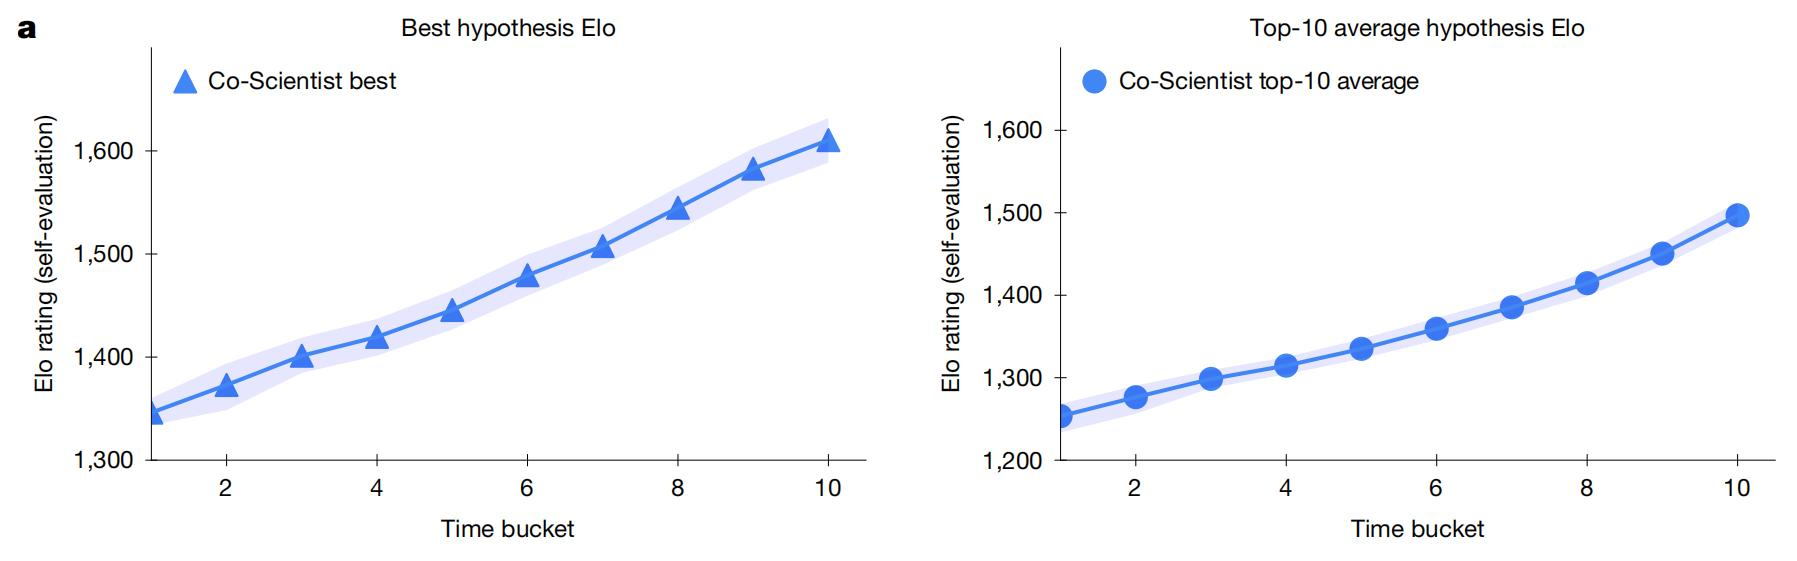
\includegraphics[width=\textwidth]{scaling_co_scientist.png}
\caption{Internal Elo ratings of the best and top-ten hypotheses over time.}
\end{figure}
\textbf{Observation:} More inference-time search improves internally
ranked hypotheses.
\smallskip

\textbf{Limits}
\begin{enumerate}
    \setlength{\itemsep}{0.25em}
    \item No saturation was observed within the tested compute range.
    \item No general quantitative law in FLOPs, tokens, or cost was established.
    \item Internal Elo ratings cannot replace experimental success rates.
\end{enumerate}
\end{frame}

% The open question is highlighted on its own page, without a block.
\setsource{\href{https://doi.org/10.1038/s41586-026-10644-y}{Co-Scientist, Nature (2026)}}
\begin{frame}[c,label=open-question]{Open Question: Emergence}
\small
\slideheading{The paper's perspective}
\medskip
The authors interpret persistent context and iterative self-improvement as an
\textbf{emergent internal model of the scientific research process}.
\smallskip
\begin{itemize}
    \setlength{\itemsep}{0.4em}
    \item \textbf{Knowledge integration:} Connect accumulated knowledge,
    synthesize information, identify gaps, and guide further hypothesis exploration.
    \item \textbf{Meta-review feedback:} Distil patterns from reviews and debates
    into subsequent prompts, improving generation and critique without parameter updates.
    \item \textbf{Adaptive orchestration:} The Supervisor uses progress statistics
    to allocate compute across agents and guide subsequent search.
\end{itemize}
\vspace{0.25cm}

\slideheading{Open question}
\medskip
{\bfseries
Can scientific intelligence emerge from this evolving internal model
of the research process?\par}
\note{The Discussion interprets context memory and iterative self-improvement
as an emergent internal model, meaning a progressively connected knowledge
state that supports information synthesis and knowledge-gap identification.
The Methods explain how research overviews guide further hypothesis generation,
how Meta-review feeds patterns from reviews and tournament debates into later
prompts, and how the Supervisor uses progress statistics to schedule agents.
These mechanisms support continued improvement with test-time compute without
updating the underlying model parameters. The internal model is not an explicit
symbolic world model; the emergence of scientific intelligence is the open
question posed on this slide, rather than an experimentally established result.}
\end{frame}

% Source page: Deepfield.md Page 9; exactly one frame.
\setsource{\href{https://www.nature.com/articles/s41586-026-10644-y}{Co-Scientist, Nature (2026)}}
\begin{frame}[t,label=md-9]{Co-Scientist: focus on generating hypotheses}
\small

\slideheading{Default Criteria}
\smallskip
\begin{enumerate}
\setlength{\itemsep}{0.65em}
    \item \textbf{Alignment} with the research goal.
    \item \textbf{Plausibility:} Check reasoning and scientific assumptions.
    \item \textbf{Novelty:} Go beyond existing knowledge; explain mechanisms.
    \item \textbf{Testability:} Validate empirically through experiments.
    \item \textbf{Safety:} Control outputs to prevent unsafe or harmful research.
\end{enumerate}
\slidenote{Additional criteria can be configured.}
\end{frame}

% Source page: Deepfield.md Page 10; exactly one frame.
\setsource{\href{https://www.nature.com/articles/s41586-026-10644-y}{Co-Scientist, Nature (2026)}}
\begin{frame}[c,label=md-10]{Scientific Exploration}
\centering
{\Large\bfseries\usebeamercolor[fg]{structure} Search + Optimization\par}
\smallskip
{\small A \textbf{combinatorial search and optimization problem}
in hypothesis space\par}
\vspace{0.7cm}

{\Large\bfseries\usebeamercolor[fg]{structure}
Exploration $\longleftrightarrow$ Exploitation\par}
\medskip
{\small Balance finite compute between new ideas and refinement.\par}
\end{frame}

% Source page: Deepfield.md Page 11; exactly one frame.
% Define the row helper outside the labeled frame so Beamer can store the frame.
\newcommand{\scientifictechniqueentry}[4]{%
    \path[fill=#2,draw=structure.fg!12,line width=0.25pt,rounded corners=2pt]
        (0.001,{#1+0.46}) rectangle (0.999,{#1-0.46});
    \node[anchor=west,inner sep=0,align=flush left,text width=0.28\textwidth,
        font=\small\bfseries,text=structure.fg] at (0.025,#1) {#3};
    \node[anchor=west,inner sep=0,align=flush left,text width=0.62\textwidth,
        font=\small,text=black] at (0.355,#1) {#4};
}
\setsource{\href{https://www.nature.com/articles/s41586-026-10644-y}{Co-Scientist, Nature (2026)}}
\begin{frame}[c,label=md-11]{New techniques to be explored...}
\small
\centering
\begin{tikzpicture}[x=\textwidth,y=1cm]
\node[anchor=west,inner sep=0,font=\footnotesize\bfseries,text=black!55]
    at (0.025,0.72) {Technique};
\node[anchor=west,inner sep=0,font=\footnotesize\bfseries,text=black!55]
    at (0.355,0.72) {Role and possible application};
\scientifictechniqueentry{0}{structure.fg!5}{World model}{%
    \textbf{Predict observable consequences} of hypotheses to support reasoning
    and experiment planning.}
\scientifictechniqueentry{-1.08}{white}{Reinforcement\\learning}{%
    \textbf{Generate hypotheses} using rewards from scientific evaluation
    and experiments.}
\scientifictechniqueentry{-2.16}{structure.fg!5}{Bayesian design}{%
    \textbf{Guide the experimental loop:} select informative tests and update
    beliefs from results.}
\scientifictechniqueentry{-3.24}{white}{Causal discovery}{%
    \textbf{Infer causal relationships} through data and interventions.}
\scientifictechniqueentry{-4.32}{structure.fg!5}{Multi-objective\\search}{%
    \textbf{Select hypotheses} by balancing novelty, plausibility,
    testability, and cost.}
\scientifictechniqueentry{-5.40}{white}{Continual learning}{%
    \textbf{Self-train the model} on validated hypotheses and research trajectories.}
\end{tikzpicture}\par
\note{These are proposed extensions to scientific reasoning and discovery.
The world model predicts observable consequences of hypotheses to support
reasoning and experiment planning.
Reinforcement learning improves the hypothesis-generation policy through
scientific evaluations and experimental feedback. Bayesian design supports
sequential experiment selection and belief updating. Causal discovery targets
causal relationships and mechanistic explanations. Continual learning is
proposed here for ongoing model self-training on validated generated
hypotheses and research trajectories.}
\end{frame}

